In this chapter, we extend the notion of bidding on concepts from a two level taxonomy to a multi-level taxonomy. We propose the notion of \textit{level-wise coverage patterns} to extract coverage patterns when a taxonomy is defined over the itemset. The notion of \textit{level-wise coverage patterns} and taxonomy based bidding has been used to propose an end-to-end framework to allocate ads to incoming search queries for sponsored search.

\section{Motivation and Basic Idea}

Search queries follow a long tail distribution with a small head of frequent (head) queries and a long tail of infrequent queries. Advertising on tail queries is hard as they occur rarely. Moreover, during ad space space auctions, advertisers are biased towards targeting head query keywords because of the individual high reach of head queries. Also, it is quite difficult for an advertiser to identify all relevant keywords from the long tail. The stated factors lead to under-utilization of ad space of tail queries which is identified as the research issue in this thesis.

In the previous chapter, we have a proposed an approach to exploit the ad space of tail keywords. We have proposed that advertisers should bid upon concepts instead of keywords in ad space auctions. We proposed to use a two level taxonomy for bidding in ad space auctions where advertisers could only bid on the first level. Through experiments, we observed that bidding on concepts shows promise with respect to ad space utilization for sponsored search. The previous approach is easy to put in practice, however, bidding on only the first level of taxonomy may not be sufficient for certain advertisers and more flexibility may be desired for certain advertising demands.


In this chapter, we propose an approach of bidding on concepts in a multi-level taxonomy instead of keywords or a two level taxonomy. During the ad space auctions, an advertiser is shown a taxonomy based on the content of his/her ad. The advertiser is then asked to select a node in the taxonomy which he/she deems the most relevant for his/her product. For example, an advertiser like \textit{Amazon.com} would be shown at taxonomy of \textit{Shopping} and based on the advertising requirements, the advertiser can select the appropriate node. If the advertisement is related to books, the advertiser would select the node \textit{Books} in the \textit{Shopping} taxonomy or if the ad is related to clothing, the advertiser would choose to bid upon \textit{Clothing} or \textit{Fashion}. Thus, the approach of bidding on a multi-level taxonomy gives more flexibility to the advertisers to target potential consumers compared to the first proposed approach.

Using the notion of bidding on a node in the taxonomy, we propose an allocation model such that groups immediate children nodes of bidding node are allocated to advertisers. Allocation of only children nodes of the bidding node is done to ensure that the allocation mechanism should consider the amount of generalization requested by the advertiser. For example, an advertiser who chose to bid upon \textit{Shopping} should not be allotted something like \{\textit{Outwear, Skirts, Shirts}\} as he would like to show his ad to a larger audience consisting of \textit{Books, Clothing, Electronics, etc.} 

To create such combinations of children nodes, the notion of coverage patterns has been employed. Coverage patterns containing children nodes of a bidden node will help in identifying mutually exclusive sets of concepts which ensure a minimum coverage and also satisfy the requirement of a maximum overlap amongst the items in the CP, thereby, reducing repetition of ad slots in the queries belonging to the concepts of the same patterns. Using the extracted coverage patterns from the query logs, a matching is performed between the coverage patterns at each node and the corresponding advertisers. 

However, in the literature the approaches proposed to extract coverage patterns \cite{srinivas2014mining} consider a flat transaction model which cannot be used to extract coverage patterns in this approach. Hence, we propose the notion of `level-wise' coverage pattern extraction when a hierarchy is present over the itemset. Using this notion of `level-wise' coverage patterns and bidding on multi-level taxonomy, we propose an end-to-end architecture to allocate ads to incoming queries. 

In the next Section, we discuss the algorithm to extract `level-wise' coverage patterns followed by the proposed framework in Section \ref{ch5Framework}, experiments in Section \ref{ch5Experiments} and a discussion in Section \ref{ch5Discussion} followed by a comparision of the two proposed approaches in Section \ref{ch5Comparison}. Section \ref{ch5Summary} summarizes the chapter.

\section{Proposed Model}
In this section, we will briefly discuss the proposed model. Compared to the standard approach of keywords based allocation in sponsored search, we have proposed to add a middle layer of coverage patterns between the advertisers and search queries. When a query is posed by a user to the search engine, it is first classified into the taxonomy nodes. The advertisers who bid upon the corresponding nodes are considered as candidate advertisers for the query's results page. Based on their bid, query-ad relevance, CTR and other parameters, the advertisers are ranked and displayed on the results page.



To extract the coverage patterns, the existing model of coverage pattern extraction proposed in the literature \cite{srinivas2014mining} cannot be employed due to the interdependence of parent-child nodes on each other. For example, if we consider a node \textit{Shopping} and its children \textit{Books,Fashion} and \textit{Electronics} then all the transactions of \textit{Books,Fashion} and \textit{Electronics} will also belong to \textit{Shopping}. Therefore, the coverage of a parent node in a transactional dataset is equal to number of transactions of its children nodes which can be stated by the following recursive relation, 
\begin{equation}
    \label{coverageFlowEQ}
    C(N_{i}) = n (\bigcup ( T(N_{i-1}) \mid \forall\ N_{i-1}:\  parent(N_{i-1}) = N_{i}))
\end{equation}


where $C(N_{i})$ is the coverage of node $N_{i}$. The coverage of $C(N_{i})$ is equal to the number of transactions of all children which is denoted by union of the transactions of the children. Equation \ref{coverageFlowEQ} shows that there is a flow of coverage from the root node to the leaf nodes in the taxonomy. Hence, the flat model of extraction of coverage patterns cannot be employed here. 




\subsection{T-Cmine: An approach to extract `level-wise' coverage patterns}

\label{Tcmine_algo}
In the proposed approach, since each session transaction contains multi-level items (query and all the taxonomy nodes related to it), the flat transaction model of coverage patterns cannot be used to extract coverage patters. In this section, we propose an approach that takes a dataset of transactions and a taxonomy defined over the items and outputs `level-wise' coverage patterns.



In \cite{srikant1997mining}, an approach to extract generalized frequent patterns has been proposed. Similarly, we propose a methodology to extract coverage patterns involving the nodes of taxonomy by extending Cmine algorithm \cite{srinivas2014mining} (also discussed in Chapter 3). For a given transactional database $\mathcal{D}$ and the taxonomy $\mathcal{T}$ which relates the items of $\mathcal{D}$, we modify each transaction by appending the ancestors of each item in the transaction to the transaction. If we apply Cmine to this modified dataset several coverage patterns containing high-level as well as low level items would be extracted. Such patterns may not be useful for ad allocation. We are interested in the coverage patterns which contains the items at the same level and satisfy the following property.

\begin{equation}
CP = \{c\ |\ c \in  (\mathcal{I} \cup \mathcal{T}) \ \&\ \forall\ c\ parent(c) = P \} \label{eq:CP2}
\end{equation}

Here, a \textit{level wise coverage pattern} is coverage pattern containing items $c$ such that all items belong to the same parent $P$. To extract level-wise coverage patterns, we propose the T-Cmine algorithm which is as follows.


\begin{algorithm}
 \textbf{Input:} $\mathcal{D}$, dataset of transactions; $\mathcal{T}$, Taxonomy defined over items of $\mathcal{D}$;\\
 \SetAlgoLined
 Compute $\mathcal{D*}$ from $\mathcal{T}$ by appending ancestors to $\mathcal{D}$;\\
 $TL_{1} := \{frequent 1\ itemsets\} $;\\
 $NO_{1} := \{frequent 1\ itemsets\} $;\\
 $C_{2} := NO_{1} \Join NO_{1}$;\\
 $TL_{2} :=$ Remove any patterns from $C_{2}$ which contain items other than sister nodes;\\
 $TL_{2} := $ Remove any patterns from $TL_{k}$ which do not satisfy $minCS$, $maxOR$ property;\\
  $NO_{2}:=$ Remove any patterns from $TL_{k}$ which do not satisfy $maxOR$ property; \\
 $k := 3$\\
 \While{$TL_{k-1} \neq \phi$ }{
  $C_{k} := NO_{k-1} \Join NO_{k-1}$;\\
  $TL_{k} := $ Remove any patterns from $TL_{k}$ which do not satisfy $minCS$, $maxOR$ property;\\
  $NO_{k}:=$ Remove any patterns from $TL_{k}$ which do not satisfy $maxOR$ property; \\
 }
 \caption{T-Cmine: Algorithm to extract Coverage Patterns with respect to a Taxonomy}
\end{algorithm}

The proposed algorithm takes a dataset $\mathcal{D}$ and a taxonomy $\mathcal{T}$ that defines the relationship amongst the items of $\mathcal{D}$. The algorithm first adds ancestors of each item in a transaction to the transaction. Then, the first set of coverage patterns ($TL_{1}$) is calculated by getting the frequent items for which relative frequency is greater than \textit{minRF}. The same set ($TL_{1}$) is also considered as Non-Overlapping Patterns set ($NO_{1}$). Using the ($NO_{1}$), candidate-2 coverage patterns are computed in the same way as Cmine algorithm. We prune all the patterns which contains other than sister nodes as stated in Equation \ref{eq:CP2}. From the pruned set, we extract patterns which satisfy both minCS and maxOR property which are the Coverage Patterns of length 2 ($TL_{2}$). In the next step, non-overlapping patterns ($NO_{2}$) are generated by sorting them in order of CS and removing any coverage patterns which don't satisfy maxOR criteria. Note that the pruning step is only required at for $k=2$ as once the patterns containing any non-sister nodes are removed, there will be no non-overlapping patterns that can be generated that contain non-sister nodes in  a CP. 
From $k=3$, for $k^{th}$ iteration of the algorithm, first candidate coverage pattern, $C_{k}$ are generated by joining $NO_{k-1}$ patterns. From $C_{k}$, any patterns which do not satisfy the minCS or maxOR are not considered to generate coverage patterns of length k, $TL_{k}$. From $C_{k}$, patterns which do not satisfy the maxOR or contain non-sisters nodes are removed and the remaining are sorted according to coverage support to generate non-overlapping sets of items of length k, $NO_{k}$. It should be noted that OR follows a `sorted' downward closure property \cite{srinivas2014mining}, and hence, the item sets of candidate sets, $C_{k}$ are sorted to obtain the corresponding non-overlapping sets $NO_{k}$. An example of the algorithm is also shown in Figure \ref{tcmine}. 

\begin{figure*}
  \centering
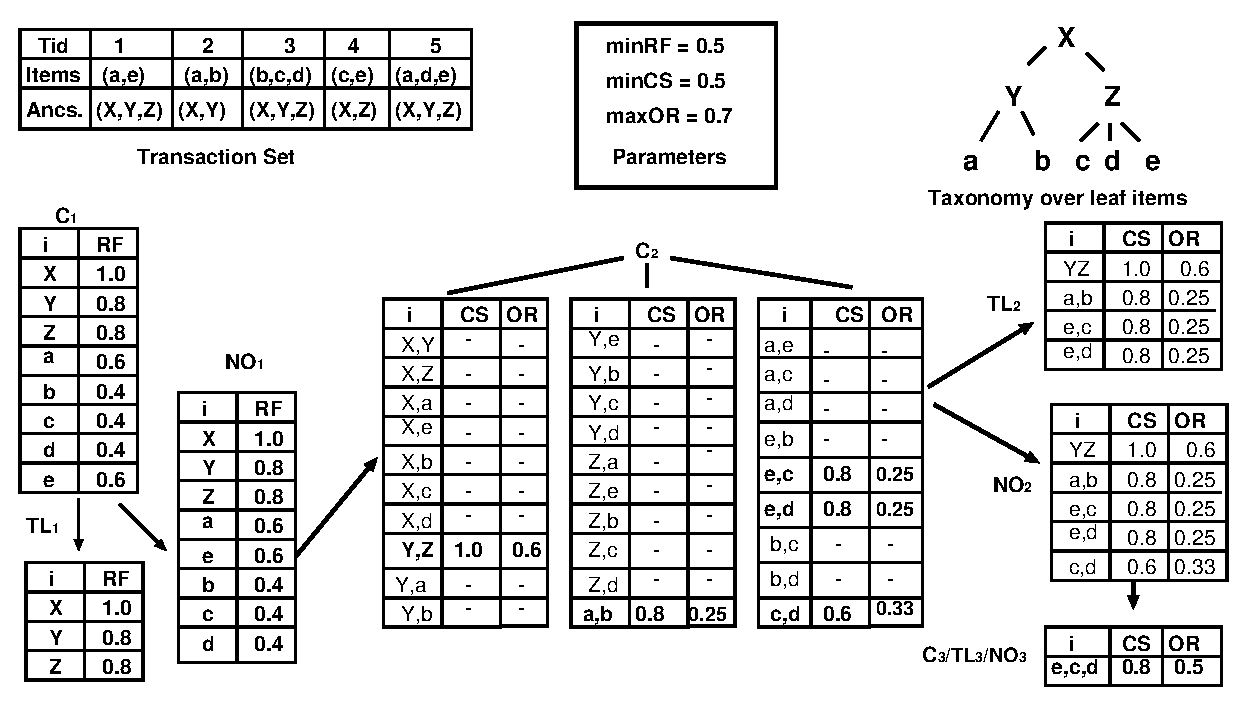
\includegraphics[scale=0.7]{visuals/T-Cmine.eps}
  \caption{Example 2: Example of T-Cmine}
  \label{tcmine}
\end{figure*}




\section{Proposed framework}

\label{ch5Framework}

In this section, we discuss the proposed model and the proposed framework as shown in Figure \ref{architecture}. We propose that in the ad space auctions, advertisers should bid upon a taxonomy instead of individual keywords. An advertiser is free to bid on any node in the taxonomy and a set of children nodes of the bidding node is allocated to the advertiser in the form of level-wise coverage patterns. When a user poses a query to the search engine, it is first classified by the bidding taxonomy into a set of nodes. For example, a query on \textit{Harry Potter} would be classified into nodes \textit{Shopping; Books; Fiction}. An advertiser who was allocated a coverage pattern containing any of these concepts would be considered to be displayed on the results page of the query - \textit{Harry Potter}. Thus, as compared to the standard sponsored search model of a bipartite graph between advertisers and queries as shown in Figure \ref{fig:adwords:model}, we add a middle layer of coverage patterns between search queries and advertisers similar to the first approach, as shown in Figure \ref{architecture} (a).


\begin{figure}
  \centering
\includegraphics[scale=0.38]{visuals/DASFAAArch.png}
  \caption{Proposed Sponsored Search Model and Architecture}
  \label{architecture}
\end{figure}

The sponsored search architecture has four major steps for query allocation to advertisers as discussed in Chapter 3. The proposed architecture also has four major online steps for allocation of incoming queries to advertisers. But, in the proposed architecture, we also exploit the knowledge extracted from the query logs in the form of coverage patterns. We discuss each step of the proposed architecture as follows.
\begin{enumerate}[label=(\roman*).]
    \item \textbf{{\em Query Analysis}}: This step is same as the standard sponsored search architecture. But, we also extract the concepts of each incoming query. For example, if the query is \textit{Harry Potter} which belongs to the taxonomy \textit{Shopping} then, it's concepts would be \textit{Shopping; Books; Fiction}.
    \item \textbf{{\em Retrieval of Relevant Advertisers}}: The input to this step is the incoming search query, its classification into the taxonomy nodes, and a matching between coverage patterns and advertisers. The matching is the output from the component where allocation of concepts to advertisers is achieved. In the next subsection, we will discuss the allocation mechanism in detail.

    \item \textbf{{\em Bidding}}: Ad space on each search query is sold by means of auctions. Each advertiser bids for the ad slots. This bid can be static or dynamic. (This step is the same as the standard sponsored search approach.) 
    
    
    \item \textbf{{\em Ranking of  Advertisers}}: Based on the bid amount and other relevant parameters like CTR and ad-query relevance, advertisers are ranked to be shown on the query's results page. (This step is also same as the standard sponsored search approach.)
\end{enumerate}



\subsection{Allocation of concepts to advertisers}

\begin{figure}
  \centering
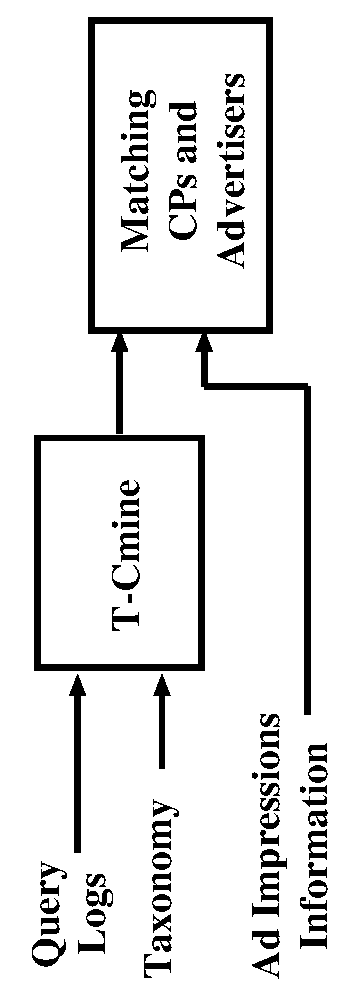
\includegraphics[scale=0.38,angle = 270]{visuals/allocationDasfaa.eps}
  \caption{Allocation of concepts to advertisers}
  \label{allocationDasfaa}
\end{figure}


In this section, we explain how concepts are allocated to advertisers. It should be noted that while considering this approach we assume the CPM (Cost Per Mille) payment mechanism, which can be easily extended to CPC (Cost Per Click) mechanism as shown in Chapter 4. The allocation process process has two main components as shown in Figure \ref{allocationDasfaa}:

\begin{enumerate}[label=(\roman*).]
    \item {\textbf{Extraction of coverage patterns using T-Cmine}}: This step takes query logs and taxonomy as input and extracts coverage patterns as explained in Section \ref{Tcmine_algo}.
    \item{\textbf{Matching coverage patterns and Advertisers}}: In this step, we take the demands of the advertisers and the coverage patterns extracted from query logs and perform a matching between the two. An allocation protocol has been proposed such that specialized requests are processed before generalized. The reason for doing a specialized-to-generalized allocation is to acknowledge that an advertiser who bids on a lower level in the taxonomy has less options of allocation compared to the advertiser who bids on a higher level. For example, an advertiser who bids on the root node can be satisfied by any choice of children nodes. However, such an allocation poses a challenge where a coverage pattern containing a parent node has to be allocated given its descendants have been allocated to advertisers. Allocation at a node should take into account if any of its descendants have been allocated as coverage of a node is sum of coverage of its descendants. Hence, impressions of a node should be modified to take into consideration if any of its descendant nodes have been allocated to the advertisers. The necessary modification to a coverage pattern if any of its descendants have been allocated to advertisers is to subtract the number of impressions allotted to the advertisers of the children of nodes contained in the respective coverage pattern. Equation \ref{CP_change} captures the necessary changes required to a coverage pattern such that for each node in the coverage pattern (denoted by $k$), count the impressions of allocated advertisers (denoted by $j$) of each descendant (denoted by $i$) and subtract it from total impressions of the coverage pattern. It should be noted that a coverage pattern is allocated to a set of advertisers if and only if it has enough impressions to satisfy the allocated advertisers. It may happen that advertisers are not allocated a coverage pattern if supply is greater than demand, and thus the following equation will never result in a negative value for the number of impressions of a coverage pattern.
    \begin{equation}
    \label{CP_change}
    CP.imp = CP.imp - \sum_{k}\sum_{ij}A_{ij}
    \end{equation}

    \end{enumerate}
    

    
\begin{figure}
  \centering
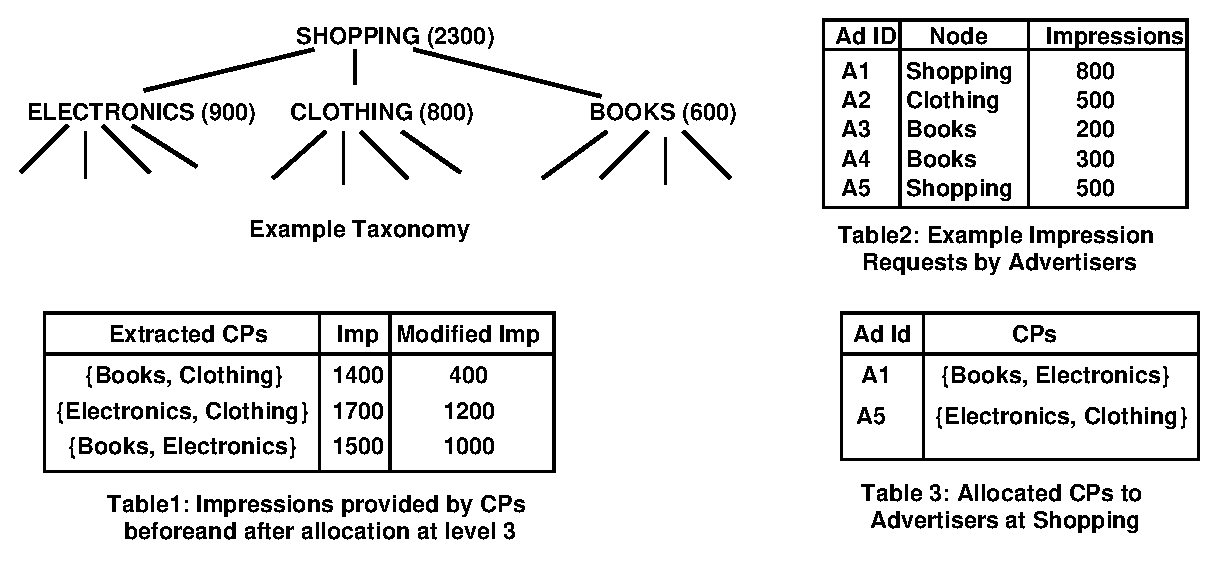
\includegraphics[scale=0.7]{visuals/ExampleAllocationDASFAA.eps}
  \caption{Example Allocation}
  \label{example_allocation}
\end{figure}


\textit{\textbf{Example 3}}: In Figure \ref{example_allocation}, we show an example allocation. We consider the top two levels of a taxonomy to show and consider advertisers who bid on the first three levels. Each advertiser bids on a node and has a demand of certain impressions at that node. Assuming allocation was done at level two i.e. for \textit{Electronics, Clothing} and \textit{Books}, we will show how it will be done for \textit{Shopping}. The node \textit{Shopping} has three children and coverage patterns pertaining to \textit{Shopping} are shown in Table 1 of Fig \ref{example_allocation}. However, as we know that allocations have been done for advertisers who chose to bid upon \textit{Books} and \textit{Clothing}, we need to adjust the impressions provided by the coverage patterns containing these two nodes. For example, the coverage pattern \textit{\{Book, Clothing\}} has 1400 initial impressions, but some advertisers were already allocated \textit{Books} and \textit{Clothing} during allocations at lower level(s). Hence, those impressions need to be subtracted i.e. 1400 - (500 + 200 + 300) = 400. Similarly, for \textit{\{Electronics, Clothing\}}, the modified number of impressions is 1200 i.e. 1700 - 500 and that of \textit{\{Books, Electronics\}} is 1000 i.e. 1500 - (200 + 300) = 1000. In the next part of this section, the matching between coverage patterns is performed considering the proposed modification.
\par
A matching is performed with advertisers as one side of the bipartite and coverage patterns as the other side. The matching is done at each node of the taxonomy where more than one advertisers choose to bid.
In order to maximize the revenue, the matching should be performed in such a way that maximum number of impressions that can be provided by the coverage patterns should be allocated. We propose the matching as an optimization problem in the same respect such that the difference between the coverage patterns and advertisers allocated to them should be minimal. For example, if an advertiser demands 100 impressions and there are two coverage patterns with impressions 150 and 200 respectively, then we chose to allocate the coverage pattern with 150 impressions. A similar case can be made when the supply of coverage patterns is 50 and 75 impressions and demand by the advertisers is 100 impressions, then the coverage pattern with 75 impressions is chosen. We frame the objective function of the matching on the same notion which is as follows. Equation \ref{impressionGoal} aims at minimizing the difference between the allocated advertising and the coverage patterns. The objective function is such that for each advertiser $Ad_{ij}$ who has been allocated the CP, $CP_{j}$ the difference between the two is minimal. Equation \ref{constraint1} lays out the constraint such that the sum of impressions of allocated advertisers does not exceed the impression provided by the coverage pattern to avoid the objective from going negative.

\begin{subequations}
\label{optiProb}
\begin{gather}
Min \ Z =  \sum_{level = d}^{0} (\sum_{j} |CP_{j}.Impressions - 
\sum_{i}^{n} (Ad_{ij}.Impressions)|) \label{impressionGoal} \\
s.t\ \ CP_{j}.Impressions >= \sum_{i=1}^{n} (Ad_{ij}.Impressions)
\label{constraint1}
\end{gather}
\end{subequations}

\textbf{Continuing Example 3} from Fig \ref{example_allocation}. From the last step, we have coverage patterns whose impressions have been updated according to allocations at their descendants. We show how the allocation is to be done for the node \textit{Shopping}. Two advertisers $A_{1}$ and $A_{5}$ chose to bid on the node \textit{Shopping}. In the proposed approach, we decide to serve the advertisers on a first-come-first-serve basis. For ad $A_{1}$, we select the coverage pattern \textit{\{Books, Electronics\}} because it has the lesser difference compared to the other node. It should be noted that now the number of impressions covered by coverage pattern \textit{\{Books, Electronics\}} has been reduced to 200 as $A_{1}$ has been allotted to it. Next, we look at ad $A_{5}$ and we see that out of the three coverage pattern, only \textit{\{Electronics, Clothing\}} has enough impressions to satisfy the advertiser and after this allocation, the number of impressions covered by \textit{\{Electronics, Clothing\}} reduces to 500. Through the example, we wanted to demonstrate how the proposed specialized-to-generalized allocation would work for advertisers who bid on \textit{Shopping} considering a set of advertisers bid on children of \textit{Shopping} and hence, the results for only $A_{1}$ and $A_{5}$ are shown. It should be noted that the matching between coverage patterns and advertisers will be one-to-many as the number of impressions that can be covered by a coverage pattern is quite high compared to demands of a single advertiser.

Considering the allocation done for Example 3, let us say a query related to the taxonomy is fired say, \textit{Harry Potter}. As shown in Figure \ref{architecture}, it will be first classified according to the taxonomy as \textit{Shopping; Books; Fiction}. Advertisers who have been allotted a coverage pattern containing any of these nodes are considered for being displayed on this query's results page i.e. $A_{1}, A_{3}, A_{4}$ and $A_{5}$ would be considered to be displayed. The decision on who out these four would be shown and in which order will be decided by the ranking mechanism which includes their bids, remaining budget etc. (As stated earlier, ranking and bidding are independent of the proposed approach.)


\section{Experiments}
\label{ch5Experiments}

\subsection{Dataset}

For the experiments, we used the CABS120k08 \cite{CABSDATA} dataset which is a collection of search queries from the AOL500k dataset along with the documents clicked, document rank, timestamps and user id. The dataset models the web document as a unit. The data set also contains the classification of the clicked document according to a concept taxonomy of four levels. From the dataset, we extracted all the queries in the form: $ <query,\ user-id,\ timestamp,\ concept\ taxonomy> $. Concept taxonomy present in the data is a four level taxonomy including the root node. Without loss of generality, we assumed that the search queries related to the documents also have the same category as the web document. The case where the same document had multiple categories, the first one was arbitrarily selected. After extracting queries, we extracted sessions of four most popular taxonomies -- {\it Arts, Health, Society} and {\it Shopping} from the dataset that had more than a single query with at least two sub-concepts of the same concept in the same session. Each session is used as a transaction to extract coverage patterns by T-Cmine as sessions form the logical boundary of searching. Table \ref{table:trainingSetStats} shows the statistics of the extracted dataset. 

\begin{table}
\centering
\caption{Search Query Dataset Statistics \label{table:trainingSetStats}}

\begin{tabular}{|c|c|c|c|c|c|} \hline
Taxonomy & Number of Nodes & Sessions & Queries  \\ \hline
Arts & 48 &7,107 & 15,317  \\ \hline
Health & 59 & 9,181 & 26,385 \\ \hline
Society & 68 & 6,471 & 13,223\\ \hline
Shopping & 79 &14,819 & 40,463 \\ \hline
Total & 254 &37,578 & 95,388 \\ \hline
\end{tabular}
\end{table}

\subsection{Implementation Methodology}

The standard sponsored search approach mentioned in \cite{mehta2007adwords} is compared with the concept-based bidding approach. We simulate advertising demands randomly in terms of impressions for five sets of advertisers having 10, 20, 30, 40 and 50 advertisers. For the standard keyword bidding, a keyword is selected as the seed for each advertiser such that the probability of selection of a keyword as the seed is proportional to its frequency in the dataset, in order to mimic the advertising demand. Followed by selection of a seed keyword, all keywords from the dataset are selected to be in the advertiser's campaign for which the Wu-Palmer similarity is more than 0.8. The number of requested impressions is randomly chosen between 100 and 1000. To simulate bid for each keyword, we consider the minimum bid as \$1.00,  the maximum bid as \$10.00 and the actual bid for each keyword is considered as the function of its relative frequency between the minimum and maximum value. For the experimental setup, we assume the bid to be paid per hundred impressions instead of per 1000 impressions as in CPM model to analyse more number of requests. The bid amount here indicated how much the advertiser is willing to pay for 100 impressions. For the concept-based bidding approach, bid of an advertiser on the concept is average of bids on all the keywords in his/her campaign.

\subsection{Performance Metrics:}Two performance metrics have been employed to compare the keywords based approach \cite{mehta2007adwords} and the proposed concept-based bidding approach.

To evaluate the utilization of ad space, we calculate the average number of unique Advertisements per Session (AS). It is calculated as the ratio of {\it Sum of Unique Advertisements of all Sessions (SUAS)} and {\it Number of Sessions with Advertisements (NSA)}. High value of AS indicates more utilization of a session, which in turn better utilization of ad space.

\begin{equation}
AS = \frac{SUAS}{NSA}
\end{equation}



We also measure the reach of each advertisement. Reach is defined as the number of users that view the ad. In this experiment, we consider reach of the ad with respect to the sessions instead of users as sessions define a logical boundary of tasks in search engines. To measure the reach,  the value of Sessions per Advertisement (SA) is calculated which is  the ratio of  {\it Number of Unique Sessions for each Ad (NUSA)} to {\it Number of Advertisements (NA)}. A higher value of the metric implies the more number of unique eye balls and thus, increasing the chances of the advertisement being viewed by {\it diverse} users.
\begin{equation}
    SA = \frac{NAS}{NA}
\end{equation}

\begin{figure}[h]
  \centering
  \subfloat[Taxonomy - Arts]{{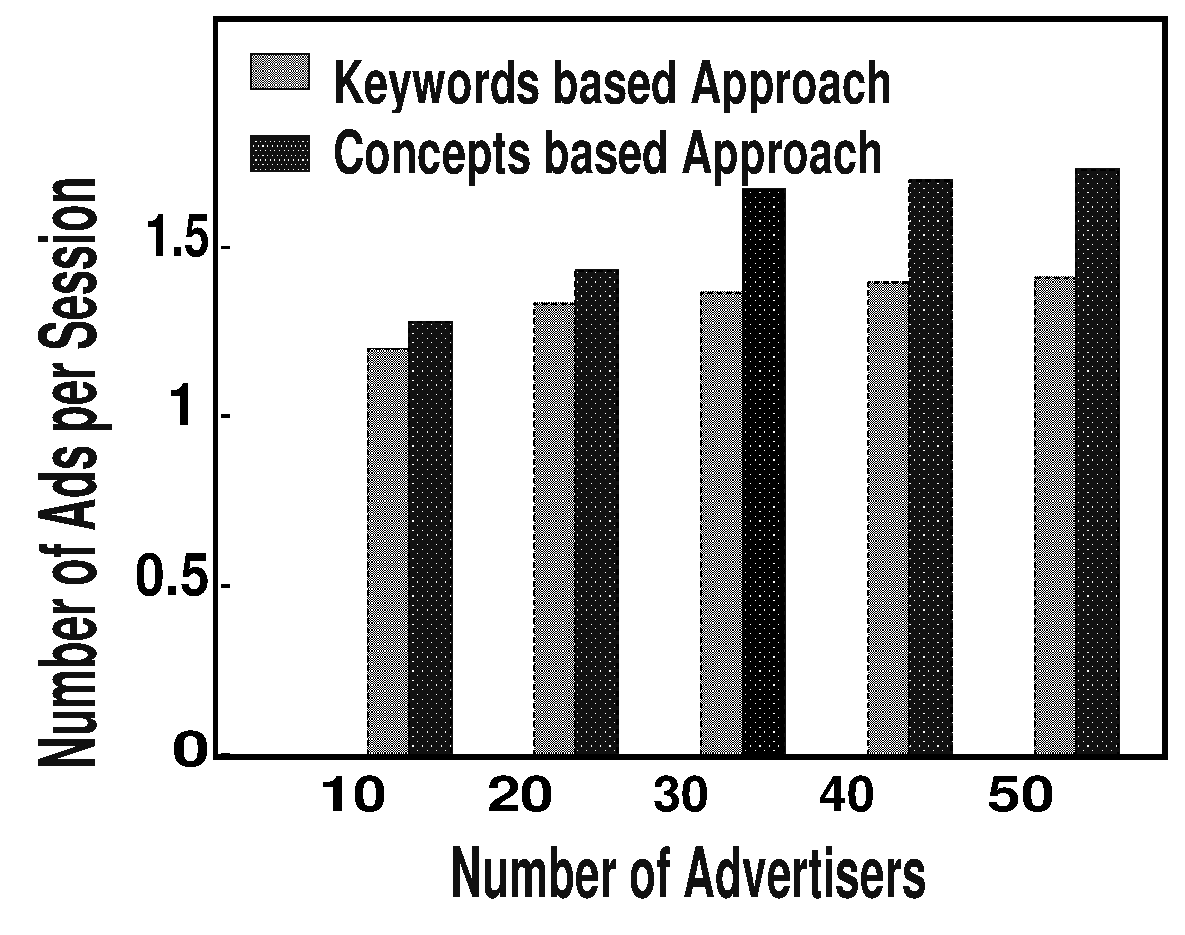
\includegraphics[height =5cm,width=5cm]{Results/arts_1.eps} }}%
  \qquad
  \subfloat[Taxonomy-Health]{{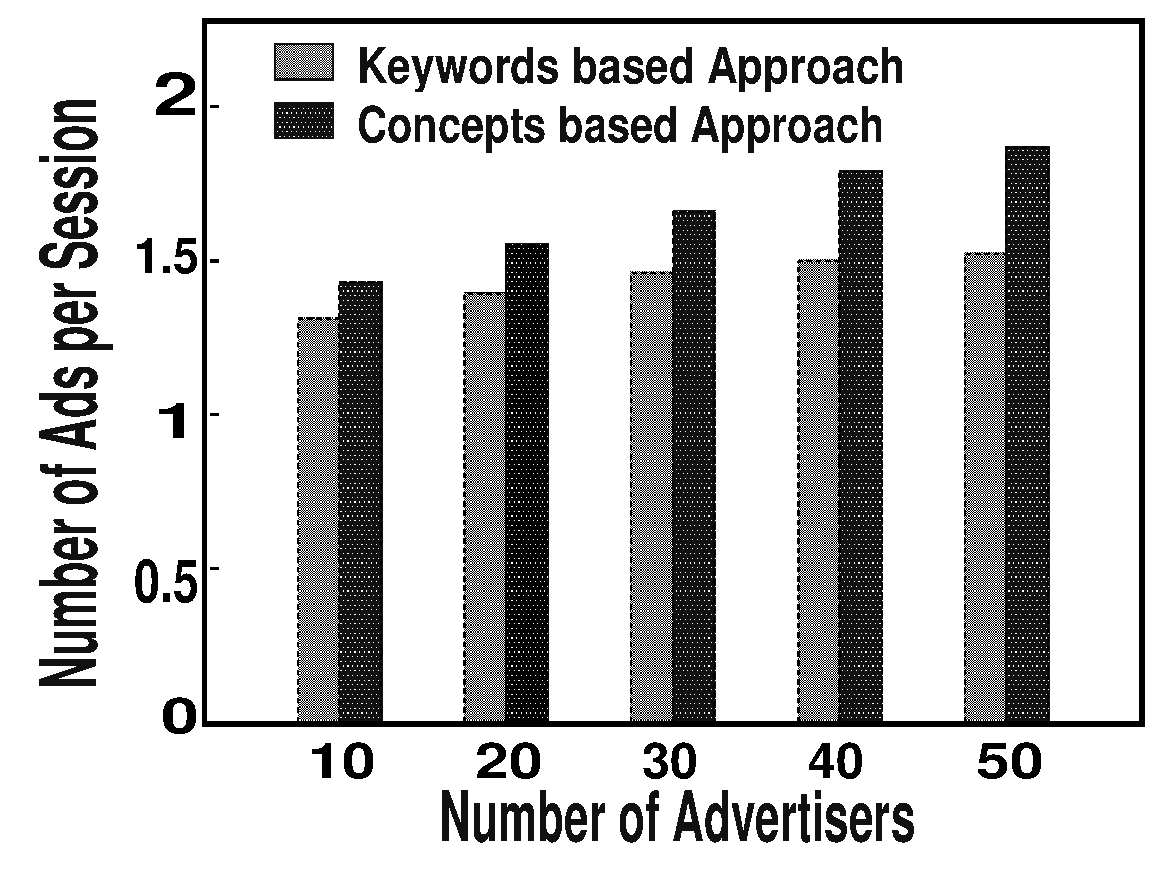
\includegraphics[height = 5cm,width=5.0cm]{Results/health_1.eps} }}%
	\qquad
	 \subfloat[Taxonomy-Shopping]{{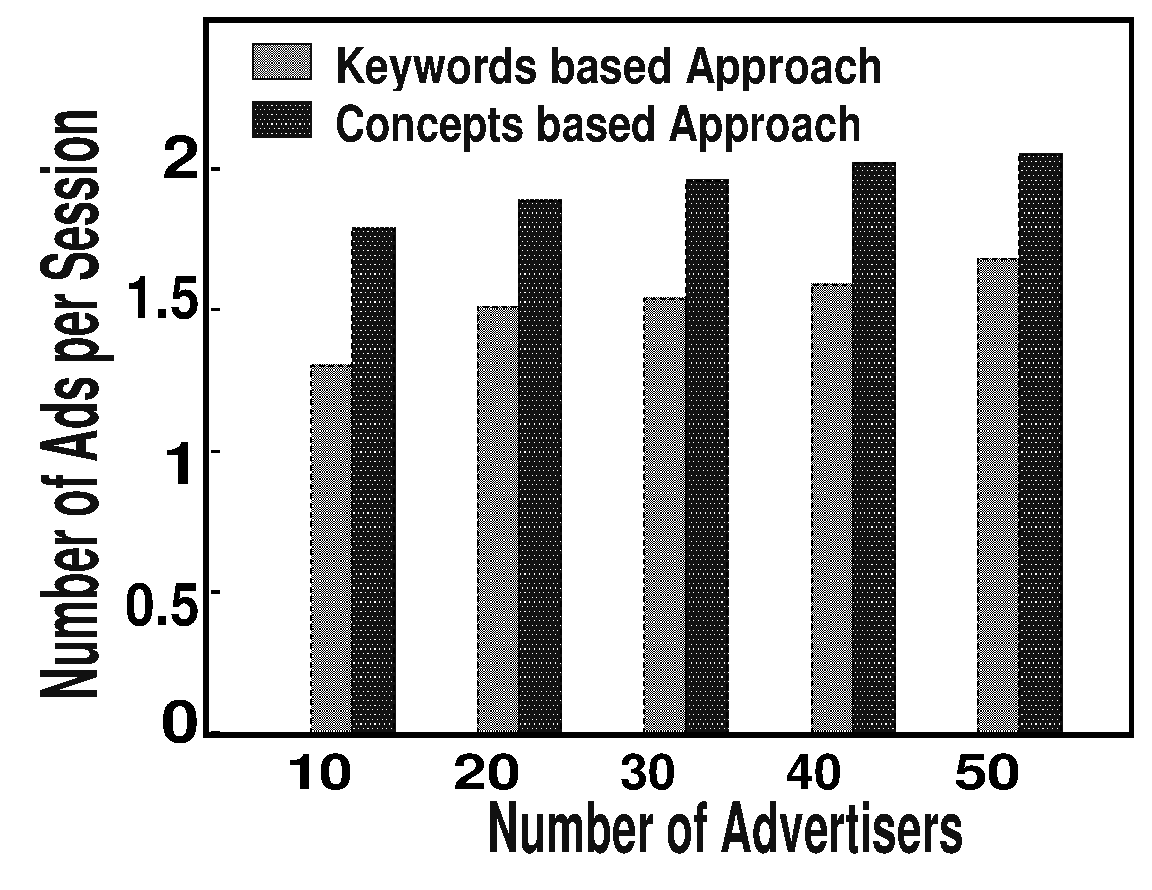
\includegraphics[height = 5cm,width=5.0cm]{Results/shopping_1.eps} }}%
 	\qquad
	 \subfloat[Taxonomy-Society]{{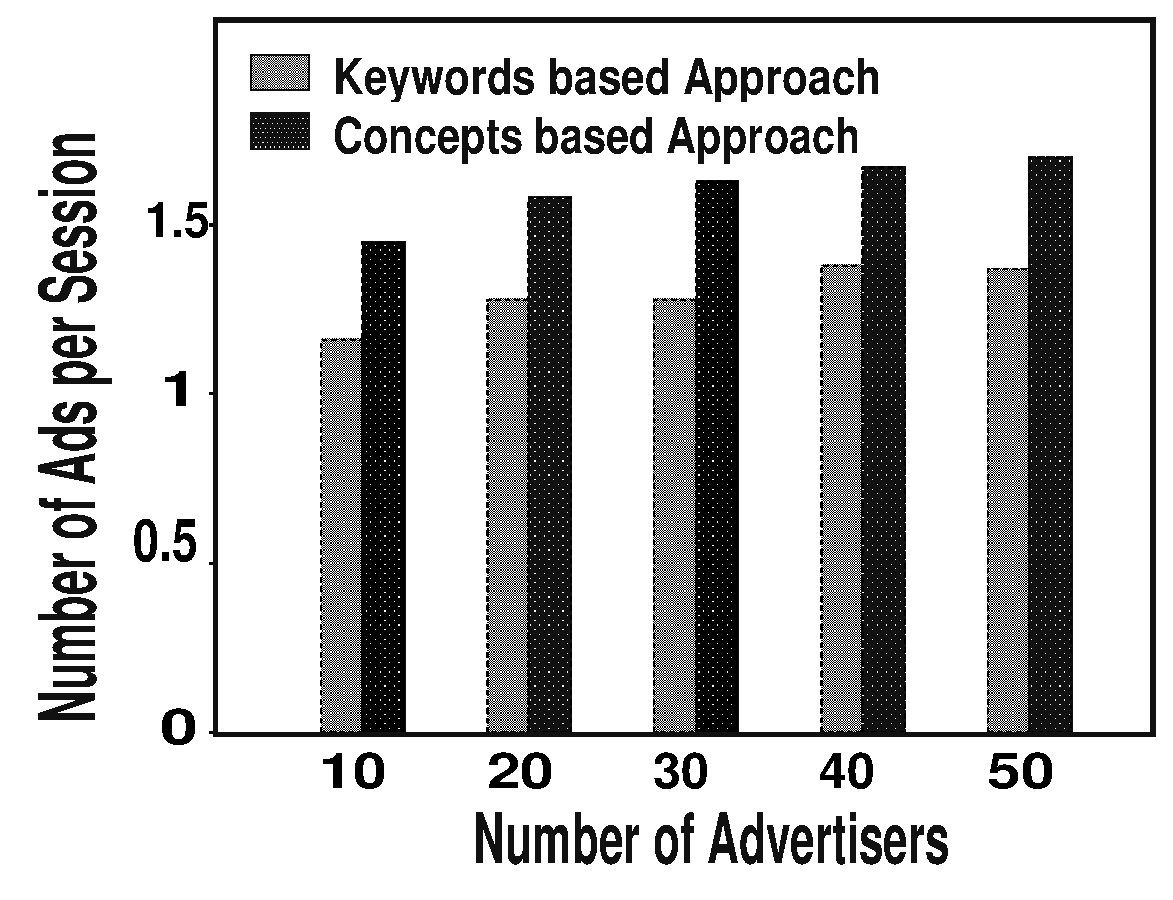
\includegraphics[height = 5cm,width=5.0cm]{Results/society_1.eps} }}%
  \caption{Performance with respect to utilization of ad space}%
  \label{fig:results1}%
\end{figure}



\subsection{Results}

\begin{figure}[h]
  \centering
  \subfloat[Taxonomy - Arts]{{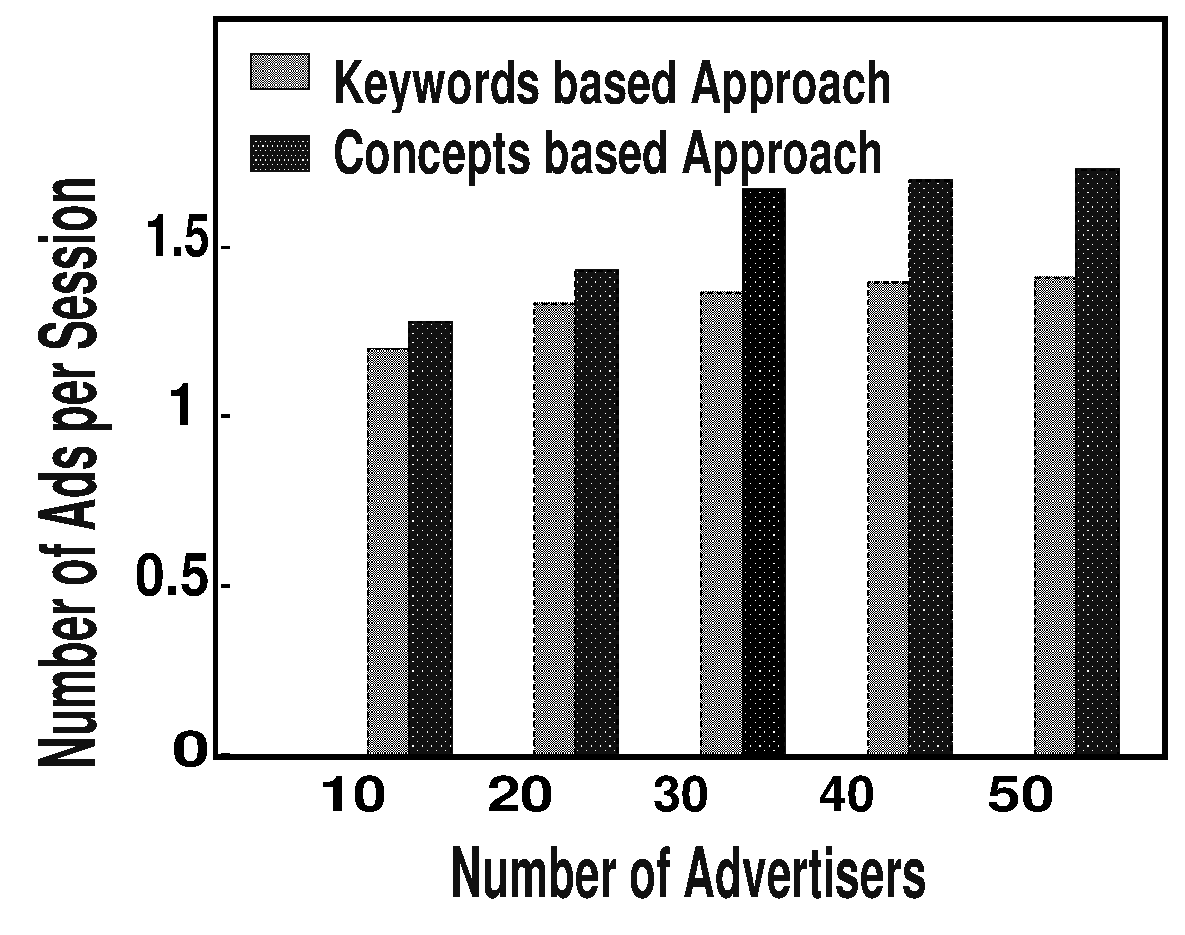
\includegraphics[height = 5cm,width=5.0cm]{Results/arts_1.eps} }}%
  \qquad
  \subfloat[Taxonomy-Health]{{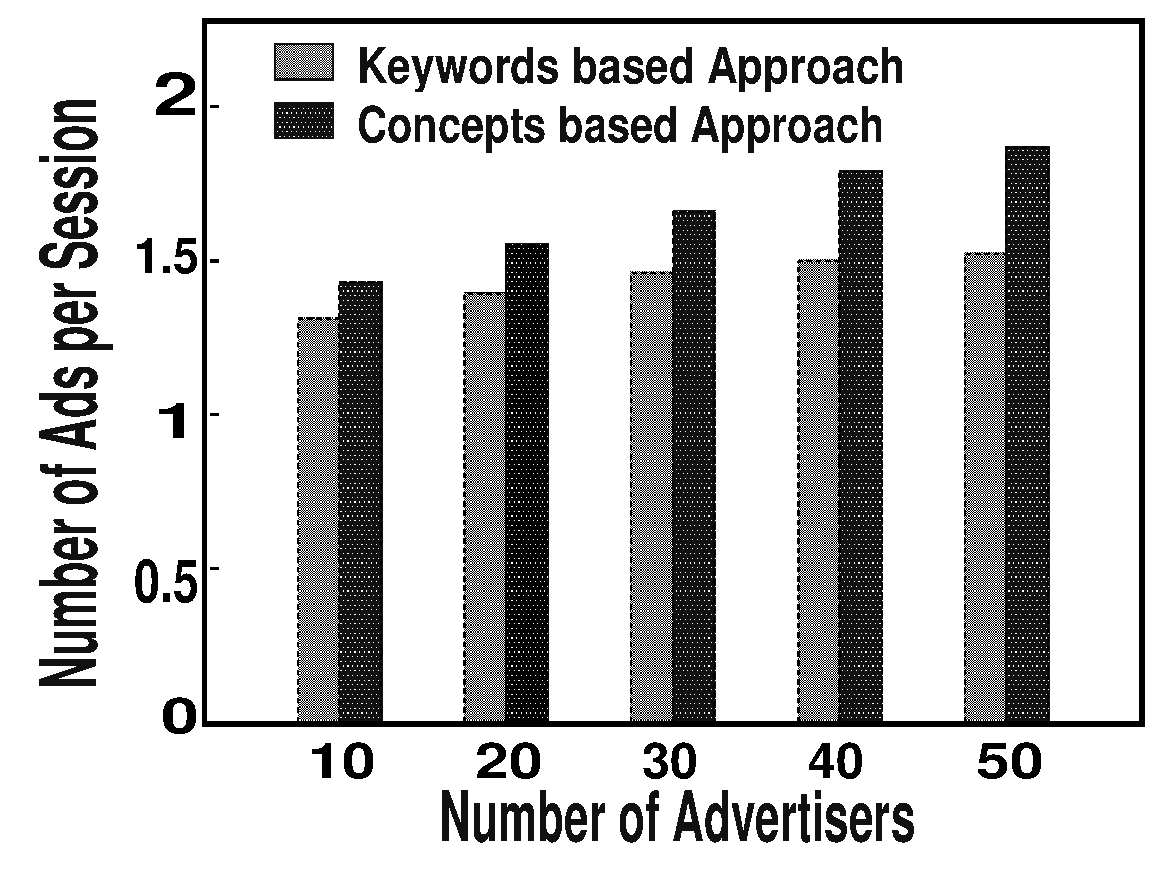
\includegraphics[height = 5cm,width=5.0cm]{Results/health_1.eps} }}%
	\qquad
	 \subfloat[Taxonomy-Shopping]{{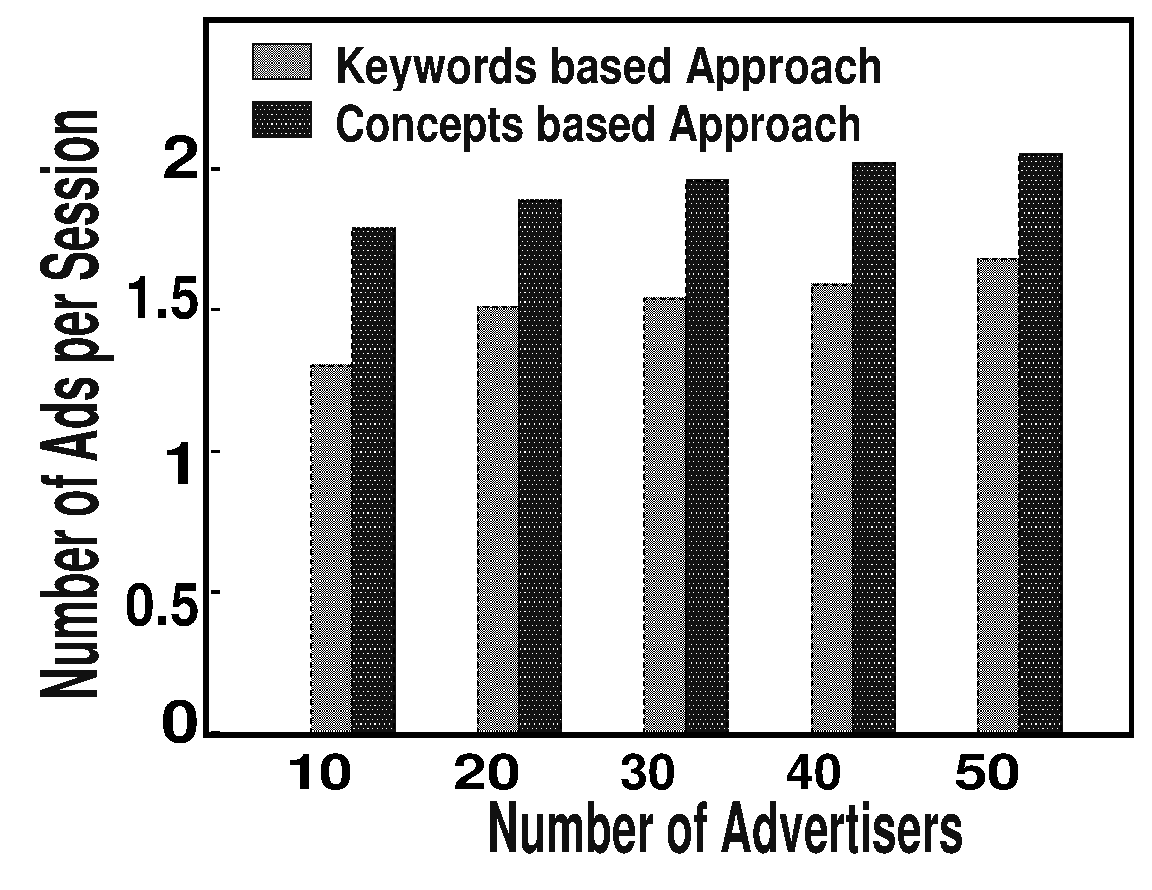
\includegraphics[height =5cm,width=5.0cm]{Results/shopping_1.eps} }}%
 	\qquad
	 \subfloat[Taxonomy-Society]{{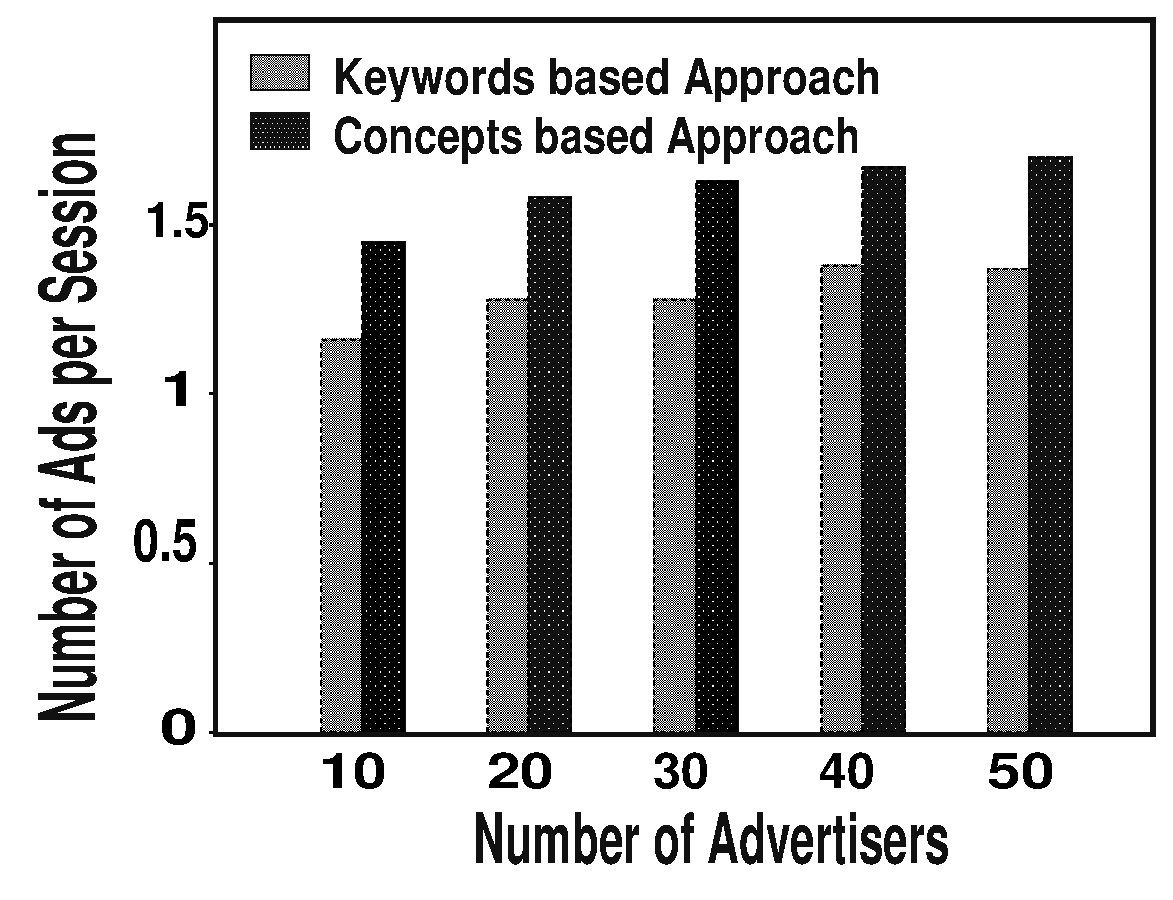
\includegraphics[height = 5cm,width=5.0cm]{Results/society_1.eps} }}%
  \caption{Performance with respect to reach of advertisers}%
  \label{fig:results2}%
\end{figure}


Figure \ref{fig:results1} reports the results with respect to ad space utilization. A fair improvement is observed in concept-based bidding mechanism. Average improvement is 19.81\% across all four taxonomies and all sets of advertisers. For individual taxonomies, average improvement for \textit{Arts} is 18.33\%, \textit{Health} is 13.74\%, \textit{Society} is 17.29\% \textit{Shopping} is 29.86\%. The improvement for \textit{Shopping} show the highest improvement by a significant margin compared to the other three taxonomies. This is because for \textit{Shopping} taxonomy average length of a session as well as distribution of nodes was higher compared to the other three taxonomies. Hence, it was possible to extract more interesting coverage patterns in the category of \textit{Shopping}. These results align in the same way for the next performance metric as well.



Figure \ref{fig:results2} shows the performance of two approaches with respect to reach of advertisements. An average improvement of 18\% was observed. For individual taxonomies, improvement for \textit{Arts} is 13.41\%, \textit{Health} is 14.83\%, \textit{Society} is 16.05\% \textit{Shopping} is 27.70\%. The results for \textit{Shopping} show significant improvements again because of the same reason as stated above.






\section{Discussion: Assumptions and Limitations}
\label{ch5Discussion}

The proposed approach has the following assumptions and limitations:
\begin{enumerate}[label=(\roman*).]

\item  We have used an external taxonomy for the experiments and we have assumed that this taxonomy is adequate enough to express the advertising requirements of the advertisers. We have also assumed that the taxonomy is appropriate enough for translating search queries into logical concepts to efficiently match advertisements to incoming queries.

\item Another assumption that we have made is that bidding on a taxonomy would be more natural than bidding on keywords. However, this needs more investigation if an advertiser would find it convenient to bid on a taxonomy as a taxonomy could very broad or could be very deep.

\item On the coverage pattern front, we have assumed the distribution of taxonomy nodes for future search queries will remain the same or change less, and hence, coverage patterns extracted today can be used tomorrow.


\item The proposed approach is also not equipped to handle query ambiguity. If the search query is ambiguous, it will be classified into multiple orthogonal taxonomy nodes and the proposed is not capable of handling that. For example, the query `Harry Potter' could belong to the node \textit{Movies} as well as \textit{Books}.

\item We have also assumed keyword distribution within each node of the taxonomy is uniform i.e. no concept is too frequent or too infrequent. This may not be true and taxonomy concepts might \textit{become popular overtime}.
    
\end{enumerate}





\section{Comparison of the proposed approaches}

\label{ch5Comparison}
Through the study presented in this chapter, we were able to show that it is possible to leverage the ad space of tail queries through extending the notion of bidding on keywords to bidding on a taxonomy.

The approach proposed in this chapter is not quantitatively comparable to the approach covered in the previous chapter as the previous approach uses a flat-concept bidding mechanism and the sub-concepts are not exposed to the advertisers but in the second approach advertisers are free to bid upon any node in the taxonomy. For example, let's consider two advertisers - \textit{Amazon} (an online shopping store) and \textit{Crosswords} (an online book store). In the first approach, both of the advertisers would bid upon Shopping. However, in the second approach, \textit{Amazon} would still bid upon Shopping but \textit{Crossword} would bid on Books. Hence, in the approach proposed in this chapter, the advertisers can choose the desired level of generalization in terms of taxonomy nodes whereas in the previous approach, the assignment is done internally. Therefore, the approaches are not quantitatively comparable. 

We discuss a qualitative comparison of both approaches in this section. Table \ref{table:comparison} states the key differences between the two proposed approaches. 

The first approach uses a two level taxonomy whereas the second approach a multi-level taxonomy for ad space auctions. 

In first approach, advertisers are only allowed to bid on the first level of the taxonomy. The second approach gives flexibility to the advertisers to bid on any node in the taxonomy and target different levels generalizations as required.





The third key difference is with respect to pricing models. A pricing model is a mechanism to decide the minimum bid amount for a given ad slot. Pricing models would remain the same or have less modifications in the first approach as each advertiser is bidding on the same level of the taxonomy. However, in the second approach advertisers can bid upon any level in the taxonomy, and thus, advertisers would bid upon different levels in the taxonomy for the same query's ad space. For example, for a query like \textit{fiction books}, advertisers who bid upon \textit{Shopping} and advertisers who chose to bid upon \textit{Books}, which is a child of \textit{Shopping}, are eligible to be shown on the results page for the query. So, pricing models are required to determine how the advertisers should be charged for a given ad slot when the bids are spread across the taxonomy.

The fourth difference in the proposed approaches is that of truthful auctions. A truthful auction aims to encourage its bidders to show their true valuations of the commodity during bidding. In the first approach, truthful auctions can be easily implemented as all advertisers are bidding at the same level of the taxonomy and all queries will be translated to the same concept for each advertiser. In the second approach, advertisers can bid on any level of the taxonomy, so it becomes crucial to make sure that the bidding is truthful. For example, if lower level nodes are generally cheaper according to the pricing model then an advertiser might bid upon several small lower nodes instead of bidding on the more relevant higher level to optimize his/her revenue.


Overall, the approach proposed in this chapter provides more flexibility to the advertisers at the cost of more complexity with respect to pricing model, auctions and allocation of advertisers to incoming queries.

\begin{table}
\centering
\caption{Comparison of the proposed approaches \label{table:comparison}}

\begin{tabular}{|c|c|c|}
\hline

\textbf{Feature} &\textbf{Approach 1} & \textbf{Approach 2} \\ \hline


\makecell{\textbf{Taxonomy Structure}} & \makecell{Flat high level concepts are\\exposed to advertisers\\for bidding} &
\makecell{Entire taxonomy of concepts\\is exposed to advertisers}\\
\hline


\makecell{\textbf{Flexibility}} & \makecell{Less flexible with respect \\to targeting potential customers} &
\makecell{More flexible with respect \\ to targeting potential customers}\\
\hline




\makecell{\textbf{Pricing Models}} & \makecell{Same pricing model could\\be used as all advertisers\\are bidding on the\\same level} &
\makecell{New pricing models need\\to be defined to address\\bidding at different levels}\\
\hline

\makecell{\textbf{Truthful Auctions}} & \makecell{Truthful auctions can be\\proven easily as bidding\\is done on the\\same level} &
\makecell{Truthful auctions have to\\be analyzed and modelled\\as bidding is allowed\\at different  granularity levels}\\
\hline



\makecell{\textbf{Complexity}} & \makecell{Easy to put in practice} &
\makecell{Relatively difficult to put\\in practice}\\
\hline


\end{tabular}
\end{table}









\section{Summary}

\label{ch5Summary}
In this chapter, we extend the previous approach of bidding on concepts instead of keywords for the ad space auctions. We proposed to generalize the previous approach from a two level taxonomy to a multi-level taxonomy. We also proposed the notion of `level-wise' coverage patterns in order to extract coverage patterns when a taxonomy is defined over the itemset. Using bidding on multi-level taxonomy and the notion of level-wise coverage patterns, we formulate an end-to-end framework for allocating ads to incoming search queries. Experiments on AOL search query logs showed improvement in performance with respect to ad space utilization and reach of the advertisements.